\documentclass[12pt]{article}
\setlength{\oddsidemargin}{0in}
\setlength{\evensidemargin}{0in}
\setlength{\textwidth}{6.5in}
%\setlength{\parindent}{0in}
%\setlength{\parskip}{\baselineskip}

\usepackage{amsmath,amsfonts,amssymb}
\usepackage{graphicx}
\usepackage{fancyhdr}
\usepackage{tikz,circuitikz,fancyvrb}
\pagestyle{fancy}


\begin{document}


\rhead{{\bf CSCI 3104 \\Problem Set 7\\ Spring 2017, CU-Boulder}}
\lhead{{\bf 
        Sam Cuthbertson (06/16)\\ 
        Grant Baker (07/23) \\ 
        Connor Hudson (05/07)}}
\renewcommand{\headrulewidth}{0.4pt}
\headheight = 43pt

\renewcommand{\arraystretch}{1.5}

\vspace{-3mm}
\begin{enumerate}

    %Q1
	\item (10 pts) \textit{Hermione needs your help with her wizardly homework. She's trying to come up with an example of a directed graph $G=(V,E)$, a 
source vertex $s\in V$ and a set of tree edges $E_{\pi}\subseteq E$ such that for each vertex $v\in V$, the unique path in the graph $(V,E_{\pi})$ from $s$ to 
$v$ is a shortest path in $G$, yet the set of edges $E_{\pi}$ cannot be produced by running a breadth-first search on $G$, no matter how the vertices are 
ordered in each adjacency list. Include an explanation of why your example satisfies the requirements. \footnote{Assistance from Luke Meszar}}\\
	
	\begin{minipage}{0.4\textwidth}
              \begin{center}
                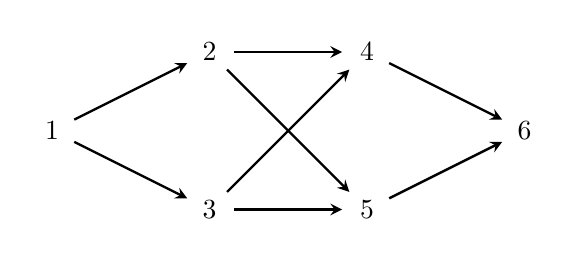
\begin{tikzpicture}[scale=1]
                    \node[circle] at (0,1) (1) {$1$};
                    \node[circle] at (2,2) (2) {$2$};
                    \node[circle] at (2,0) (3) {$3$};
                    \node[circle] at (4,2) (4) {$4$};
                    \node[circle] at (4,0) (5) {$5$};
                    \node[circle] at (6,1) (6) {$6$};
                  
                    \draw[->,>=stealth,line width=0.3mm] (1) -- (2);
                    \draw[->,>=stealth,line width=0.3mm] (2) -- (4);
                    \draw[->,>=stealth,line width=0.3mm] (4) -- (6);
                    \draw[->,>=stealth,line width=0.3mm] (1) -- (3);
                    \draw[->,>=stealth,line width=0.3mm] (3) -- (5);
                    \draw[->,>=stealth,line width=0.3mm] (5) -- (6);
                    \draw[->,>=stealth,line width=0.3mm] (2) -- (5);
                    \draw[->,>=stealth,line width=0.3mm] (3) -- (4);
                \end{tikzpicture} \\
                Graph with all edges
              \end{center}
            \end{minipage}
            \hfill
            \begin{minipage}{0.4\textwidth}
              \begin{center}
                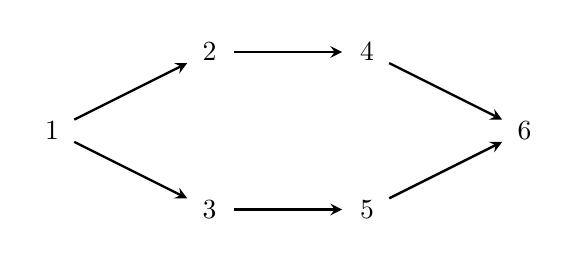
\begin{tikzpicture}[scale=1]
                    \node[circle] at (0,1) (1) {$1$};
                    \node[circle] at (2,2) (2) {$2$};
                    \node[circle] at (2,0) (3) {$3$};
                    \node[circle] at (4,2) (4) {$4$};
                    \node[circle] at (4,0) (5) {$5$};
                    \node[circle] at (6,1) (6) {$6$};
                  
                    \draw[->,>=stealth,line width=0.3mm] (1) -- (2);
                    \draw[->,>=stealth,line width=0.3mm] (2) -- (4);
                    \draw[->,>=stealth,line width=0.3mm] (4) -- (6);
                    \draw[->,>=stealth,line width=0.3mm] (1) -- (3);
                    \draw[->,>=stealth,line width=0.3mm] (3) -- (5);
                    \draw[->,>=stealth,line width=0.3mm] (5) -- (6);
                \end{tikzpicture} \\
                Tree with edges $E_{\pi}$, using s = 1
              \end{center}
            \end{minipage}
    
    \vspace{7mm}
	\begin{minipage}{0.4\textwidth}
            \begin{center}
                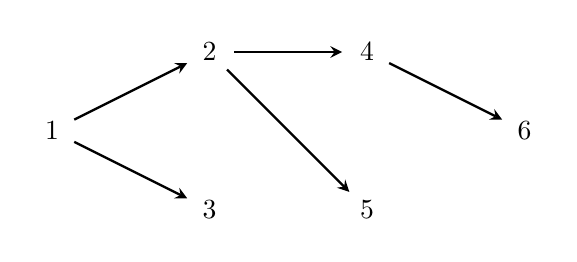
\begin{tikzpicture}[scale=1]
                    \node[circle] at (0,1) (1) {$1$};
                    \node[circle] at (2,2) (2) {$2$};
                    \node[circle] at (2,0) (3) {$3$};
                    \node[circle] at (4,2) (4) {$4$};
                    \node[circle] at (4,0) (5) {$5$};
                    \node[circle] at (6,1) (6) {$6$};
                  
                    \draw[->,>=stealth,line width=0.3mm] (1) -- (2);
                    \draw[->,>=stealth,line width=0.3mm] (2) -- (4);
                    \draw[->,>=stealth,line width=0.3mm] (4) -- (6);
                    \draw[->,>=stealth,line width=0.3mm] (1) -- (3);
                    \draw[->,>=stealth,line width=0.3mm] (2) -- (5);
                \end{tikzpicture} \\
                A Possible BFS Tree
              \end{center}
            \end{minipage}
            \hfill
            \begin{minipage}{0.4\textwidth}
              \begin{center}
                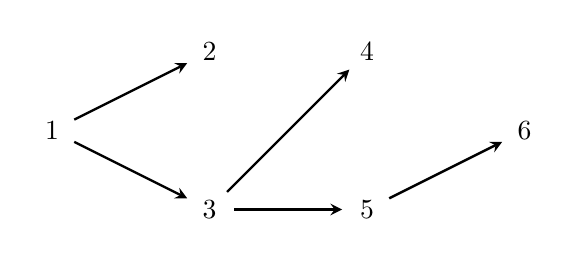
\begin{tikzpicture}[scale=1]
                    \node[circle] at (0,1) (1) {$1$};
                    \node[circle] at (2,2) (2) {$2$};
                    \node[circle] at (2,0) (3) {$3$};
                    \node[circle] at (4,2) (4) {$4$};
                    \node[circle] at (4,0) (5) {$5$};
                    \node[circle] at (6,1) (6) {$6$};
                  
                    \draw[->,>=stealth,line width=0.3mm] (1) -- (2);
                    \draw[->,>=stealth,line width=0.3mm] (3) -- (4);
                    \draw[->,>=stealth,line width=0.3mm] (1) -- (3);
                    \draw[->,>=stealth,line width=0.3mm] (3) -- (5);
                    \draw[->,>=stealth,line width=0.3mm] (5) -- (6);
                \end{tikzpicture} \\
                Another Possible BFS Tree
              \end{center}
            \end{minipage}
            
    \vspace{7mm}        
    Our set of edges $E_{\pi}$ cannot be found by BFS due to the way that BFS examines all edges from a given vertex exhaustively, leading to the behaviour 
shown above. With our graph and beginning at node 1, BFS would examine 2 and 3 at depth one, then moving on to examine either 2 or 3 for nodes at depth two. 
In that process, it would find the paths from 2 {\bf OR} 3 to 4 and 5, thus missing at least one of the edges in our set $E_{\pi}$. \\
    
    This behaviour is shown twice above, once where node 2 is encountered first and once where node 3 is encountered first. It's worth noting that something 
similar would happen with the path to 6, where BFS could encounter either 4 or 5 first, but permutations of that are trivial and thus not shown.

    \newpage
    %Q2
	\item (10 pts) \textit{Review the material on depth-first spanning forests in Chapter 22.3 of the textbook. Then, consider the directed graph $G$ 
defined by the edge list}
	\vspace{-2mm}
	\begin{align}
	G=\{ (1,2),(1,4),(1,8),(2,3),(3,1),(4,8),(5,2),(5,6),(6,2),(6,3),(6,5),(7,4),(8,7) \} \nonumber 
	\end{align}
	\begin{enumerate}
	\item \textit{Draw the depth-first spanning forest, including and identifying all tree, back, forward, and cross edges. (If you prefer, you can 
identify the forward, back, and cross edges in separate lists instead of trying to draw and label them.)\footnote{Slight collaboration with Adam Smrekar}} \\
	\begin{center}
	    \begin{minipage}{0.2\textwidth}
    	    \begin{center}
        	    \color{cyan}{Cross Edges}\\
    	        \color{red}{Back Edges}\\
    	        \color{blue}{Forward Edges}
	        \end{center}
	    \end{minipage}
	    \hfill
	    \begin{minipage}{0.6\textwidth}
    	    \begin{center}
    	    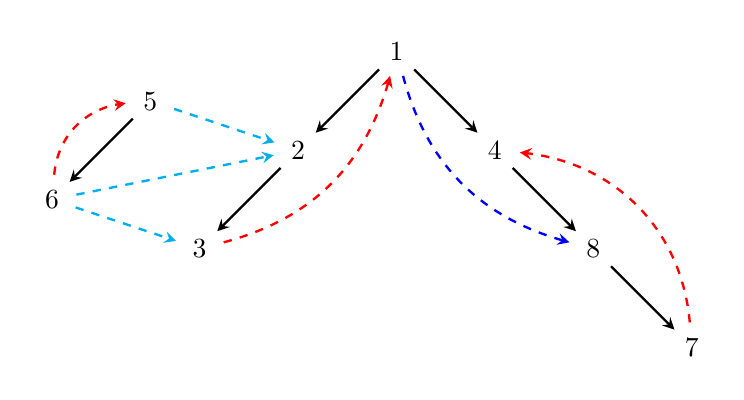
\begin{tikzpicture}[scale = 1.25]
    	        \node[circle] at (5,5) (1) {$1$};
    	        \node[circle] at (4,4) (2) {$2$};
    	        \node[circle] at (3,3) (3) {$3$};
    	        \node[circle] at (6,4) (4) {$4$};
    	        \node[circle] at (7,3) (8) {$8$};
    	        \node[circle] at (8,2) (7) {$7$};
    	        \node[circle] at (2.5,4.5) (5) {$5$};
    	        \node[circle] at (1.5,3.5) (6) {$6$};
    	        
    	        \draw[->,>=stealth,line width=0.3mm] (1) -- (2);
    	        \draw[->,>=stealth,line width=0.3mm] (2) -- (3);
    	        \draw[->,>=stealth,line width=0.3mm] (5) -- (6);
    	        \draw[->,>=stealth,line width=0.3mm] (1) -- (4);
    	        \draw[->,>=stealth,line width=0.3mm] (4) -- (8);
    	        \draw[->,>=stealth,line width=0.3mm] (8) -- (7);
    	        
    	        \draw[->,dashed,>=stealth,line width=0.3mm,red] (7) edge[bend right=40] (4); 
    	        \draw[->,dashed,>=stealth,line width=0.3mm,red] (3) edge[bend right=30] (1); 
    	        \draw[->,dashed,>=stealth,line width=0.3mm,blue] (1) edge[bend right=30] (8);
    	        \draw[->,dashed,>=stealth,line width=0.3mm,red] (6) edge[bend left=40] (5); 
    	        \draw[->,dashed,>=stealth,line width=0.3mm,cyan] (5) edge (2); 
    	        \draw[->,dashed,>=stealth,line width=0.3mm,cyan] (6) edge (2); 
    	        \draw[->,dashed,>=stealth,line width=0.3mm,cyan] (6) edge (3); 
    	    \end{tikzpicture}
    	    \end{center}
	    \end{minipage}
	\end{center}

	\item \textit{List all the strong components in $G$.}\\
	The smallest strong element is nodes 5 and 6, the second element is nodes 1, 2 and 3, while the last element is nodes 4, 8 and 7.
	
	\end{enumerate}
	

    \newpage
    %Q3
	\item (30 pts) \textit{Prof. Snape claims that when an {\em adjacency matrix} representation is used, most graph algorithms take $\Omega(V^{2})$ time, 
but there are some exceptions.}

	\textit{One such exception, Snape claims, is determining whether a directed graph $G$ contains a \textit{black hole}, which is defined as a vertex 
with in-degree $|V|-1$ (i.e., every other vertex points to this one) and out-degree $0$. Snape sourly claims that this determination can be made in time 
$O(V)$, given an adjacency matrix for $G$. Prove that Snape is correct.}\\
	
	\textit{Hint: This is a ``proof by algorithm'' question. That is, describe and analyze an algorithm that yields the correct answer on every type of 
input (``yes'' when a black hole exists and ``no'' when it does not). Think about the boundary cases, where it is the most difficult to distinguish a correct 
``yes'' from a correct ``no.''}\\
	
    We can find the black hole by noting that if there is an edge from vertex $i$ to $j$, then $i$ cannot be a black hole. Also, if there is not an edge from 
vertex $i$ to $j$, then $j$ cannot be a black hole.\\
    
    So, given the adjacency matrix, we iterate through the columns left to right, starting at the second element in the first row. If an element is a $1$, 
then we jump to the row of the current column before going to the next column. Otherwise, continue directly right. This represents a process of elimination 
through which we eliminate one vertex in each column of the matrix.\\
    
    After reaching the last column, our current row is a potential black hole. We then iterate through the row to ensure it is all $0$s, and the corresponsing 
column to ensure it is all $1$s except on the diagonal.\\
    
    Also note that no graph can contain two black holes since there would be a conflict in the edge between the two vertices.\\
    
    Below is a pseudocode implementation of the algorithm, and a Python implementation is included in Appendix \ref{app:3}:

\newpage    
\begin{small}
\begin{verbatim}
containsBlackHole(G):           // G is a |V|x|V| adjacency matrix
    i = 0                       // 0-indexed
    for j in 1...|V|-1:                      // |V|-1 iterations
        if G[i][j] == 1:
            i = j
    if 1 in G[i]:               // ith row,     |V| iterations
        return No 
    else if 0 in {G[All][i] except ith row}: // |V|-1 iterations
        return No               // ith column except diagonal
    else:
        return Yes
\end{verbatim}
\end{small}
	
	The algorithm only iterates over $|V|-1$ items when going through the matrix, $|V|$ items when checking the validity of the row, and $|V|-1$ items 
when checking the validity of the column, so it has a total runtime of $3|V|-2$, or $O(V)$.\\
	
	Notably, the runtime would be asymptotically larger if we could not check whether an edge between two nodes existed in more than $O(1)$ time, which is 
a feature of the adjacency matrix.
	
% 	\textsf{Dibs -G}
	

    \newpage
    %Q4
	\item (30 pts) \textit{Deep in the heart of the Hogwarts School of Witchcraft and Wizardry, there lies a magical Sphinx that demands that any 
challenger efficiently convert directed multigraphs into undirected simple graphs. If the wizard can correctly solve a series of arbitrary instances of this 
problem, the Sphinx will unlock a secret passageway.} 
	
	\textit{Let $G=(E,V)$ denote a directed multigraph. An undirected simple graph is a $G'=(V,E')$, such that $E'$ is derived from the edges in $E$ so 
that (i)~every directed multi-edge, e.g., $\{(u,v),(u,v)\}$ or even simply $\{(u,v)\}$, has been replaced by a single pair of directed edges $\{(u,v),(v,u)\}$ 
and (ii)~all self-loops $(u,u)$ have been removed.}


	\textit{Describe and analyze an algorithm (explain how it works, give pseudocode if necessary, derive its running time and space usage, and prove its 
correctness) that takes \mbox{$O(V+E)$} time and space to convert $G$ into $G'$, and thereby will solve any of the Sphinx's questions. Assume both $G$ and 
$G'$ are stored as adjacency lists.}
	
	A solution for this problem would be to iterate over the adjacency list for every vertex, ignoring self-adjacency, and adding undirected edges 
wherever there is \textit{any} edge between two vertices, as shown in the pseudocode below. We then iterate over the resulting adjacency lists, coloring each 
vertex based on whether we have previously seen it, deleting an item from the list if we have seen that vertex before.\footnote{Help from Luke Meszar}
	
	\begin{small}
	\begin{verbatim}
	for each vertex v in G: // O(V)
	    for each i in Adj[v]:
	        if i == v: // self-adjacent - ignore. O(1)
	            do nothing
	        else:
	            // Create an undirected edge between i and v
	            Adj[i].add(v) // O(1)
	            Adj[v].add(i) // O(1)
	        
	for each vertex v in G': // O(v)
	    colordict = [WHITE for all v in G']
	    for each i in Adj'[v]:
	        if colordict[i] == WHITE: // O(1)
	            colordict[i] = BLACK // O(1)
	        
	        if colordict[i] == BLACK: // O(1)
	            delete i // O(1)
	        
	\end{verbatim}
	\end{small}
	
	We use $O(V + E)$ space to store G, and $O(V + E') = O(V + E)$ space to store G'. We also use $O(V)$ space for the color dictionary. Thus, our space 
usage is $O(V + E)$.
	
	The running time is $O(V + E)$ since each of the two loops adds a factor of $O(V)$ and the iterations over the adjacency lists take a \textit{total} 
of $O(E)$ operations. Thus, the running time is $O(V + E)$.
	
	Once the algorithm has finished, there are no duplicate edges, so our graph is simple. In the 'else' statement, we symmetrically add to the adjacency 
lists so our graph is by definition undirected. Putting these together shows that our resulting graph is simple and undirected, satisfying the problem's 
constraints.

    \newpage
    %Q5
	\item (20 pts) \textit{Crabbe and Goyle are at it again. Crabbe thinks min-heaps are for muggles and instead wants to use a max-heap to run the SSSP 
algorithm. He writes the following code on the whiteboard and bounces up and down in excitement, because he thinks he's going to get an algorithm named after 
himself. \footnote{Collaboration with Adam Smrekar}}
\begin{small}
\begin{verbatim}
CrabbeSSSP(G, s) :
     # G is an adjacency list with n nodes and m directed edges
     H = empty max-heap
     for each node i {
        d[i] = INF
        insert i into H with key d[i]
     }
     d[s] = 0
     insert s into H with key d[s]
     while (H is empty) {
        v = extractMin(H)
        for each edge (v,u) {
           if (v,u) is tense {
              Relax(v,u)
              insert v into H with key d[v]
           }
     }}
\end{verbatim}
\end{small}

\textit{Hermione snorts, saying this is hardly an \textit{efficient} algorithm, and besides, it has one or more bugs in it (she won't say which!).}
	
	\begin{enumerate}
	\item \textit{Identify the bug(s) in Crabbe's algorithm, explain why they would lead to an incorrect algorithm, and give the corrected pseudocode.}\\
	
    First, the line {\tt for each node i} should be {\tt for each node i $\neq$ s}, as s will have it's distance set to 0, and be added to H, below this 
point. Second, the line {\tt while (H is empty)} should be {\tt while (H is not empty)} as H begins full and is emptied as the algorithm continues. Finally, 
the line {\tt insert v into H with key d[v]} should be {\tt insert u into H with key d[u]} as inserting the item we just extracted can lead to a boundless 
loop. The corrected pseudocode is given below:\\

\begin{verbatim}
CrabbeSSSP(G, s) :
     # G is an adjacency list with n nodes and m directed edges
     H = empty max-heap
     for each node i != s {
        d[i] = INF
        insert i into H with key d[i]
     }
     d[s] = 0
     insert s into H with key d[s]
     while (H is not empty) {
        v = extractMin(H)
        for each edge (v,u) {
           if (v,u) is tense {
              Relax(v,u)
              insert u into H with key d[u]
           }
     }}
\end{verbatim}

	\item \textit{Analyze the corrected version of Crabbe's algorithm to determine is running time, and comment on why Crabbe will probably not get an 
algorithm named after him.}\\
    Starting at the top, where n is the number of vertexes and m is the number of edges:
    \begin{itemize}
        \item Allocating an empty max heap is O(1)
        \item Iterating over the list of vertexes will be a factor of n
        \begin{itemize}
            \item Setting an element in an array is O(1)
            \item Inserting an element into a heap is O($\log n$)
        \end{itemize}
        \item Setting an element in an array is O(1)
        \item Inserting an element into the heap is O($\log n$)
        \item As the heap is full of all vertexes, this loop is a factor of n
        \begin{itemize}
            \item Extracting the minimum element from a max heap is O(n)
            \item Iterating over all the edges from a vertex would be a factor of an additional m for this loop.
            \begin{itemize}
                \item Inserting an item into a max heap is O($\log n$)
            \end{itemize}
            %aaaa
        \end{itemize}
    \end{itemize}
    \vspace{5mm}
    Putting it all together, we get
    \begin{align*}
        &O(1) + nO(\log n) + O(\log n) + nO(n) +nO(m\log n)\\
        &O(n\log n + n(n + m\log(n)))\\
        &O((n+nm)\log n + n^2)\\
        &O(n^2)
    \end{align*}
    
    Note that the cost of finding the minimum of a max-heap dominates with a runtime of $O(n)$, an action which we perform $O(n)$ times.
    
	
	\end{enumerate}


    \newpage
    %Q6
	\item (15 pts extra credit) \textit{Professor Snape has provided the young wizard Hermione with three magical batteries whose sizes are 12, 7, and 6 
morts, respectively. (A \textit{mort} is a unit of wizard energy.) The 7-mort and 6-mort batteries are fully charged (containing 7 and 6 morts of energy, 
respectively), while the 12-mort battery is empty, with 0 morts. Snape says that Hermione is only allowed to use, repeatedly, if necessary, the \textit{mort 
transfer spell} when working with these batteries. This spell transfers all the morts in one battery to another battery, and it halts the transfer either when 
the source battery has no morts remaining or when the destination battery is fully charged.}
	
	\textit{Snape condescendingly challenges Hermione to determine whether there exists a sequence of mort-transfer spells that leaves exactly 2 morts 
either in the 7-mort or in the 6-mort battery.}
	\begin{enumerate}
	\item \textit{Hermione knows this is actually a graph problem. Give a precise definition of how to model this problem as a graph, and state the 
specific question about this graph that must be answered.}\\
	
	This problem can be transformed into a graph where every node is an ordered triple. For example, a node $(0,7,6)$ can represent the configuration 
where the 12-battery has 0 morts, the 7-battery has 7 morts, and the 6-battery has 6 morts.\\
	
	Each edge then represents the mort transfer spell from one battery to another. For example, the node $(7,0,6)$ is adjacent to $(0,7,6)$ because we can 
transfer the 7 morts to the 12-mort battery with the spell.\\
	
	The question that must be answered is then: \textbf{Is there a path from the node $(0,7,6)$ to a node of the form $(x,2,11-x)$ or $(x,11-x,2)$?}\\
	
	\item \textit{What algorithm should Hermione apply to solve the graph problem?}\\
	
	This problem is easily solved with a Breadth-First Search algorithm, where the terminating condition is that the second or third component of the node 
is $2$.\\
	
	\newpage
	\item \textit{Apply that algorithm to Snape's question. Report and justify your answer.} \\
	
	We implemented the BFS algorithm for this specific problem in Python, attached in Appendix \ref{app:6}. One such answer is the path:
	\[
	(0,7,6)\rightarrow(7,0,6)\rightarrow(12,0,1)\rightarrow(5,7,1)\rightarrow(5,2,6)
	\]
	
	This corresponds to the series of mort transfer spells, where $(x\rightarrow y)$ represents the transfer from the battery of capacity $x$ to the 
battery of capacity $y$:
	\[
	    (7\rightarrow12), (6\rightarrow12), (12\rightarrow7), (7\rightarrow6)
	\]

    Or, of course, we could give Voldemort a 2-volt battery, since only Voldemort knows the \textit{Volt-to-Mort} spell.\footnote{Joke from Matt Maierhofer}
	
	
	
% 	We obviously need to justify the answer. Justifying the answer is 
% 	what you do! People always ask me, "Are you going to justify this?" I think, of course! I'll justify it. Justifying it is what you need to do. It 
makes sense. It's important. I have the best justifications. BELIEVE ME. The Democrats don't justify anything. ISIS won't justify their answers. WE NEED TO 
MAKE AMERICA JUSTIFY AGAIN!
% 	#MAJA
	\end{enumerate}
	
% 	\textsf{dibs -G}

\end{enumerate}

\newpage
\appendix
\section{Problem 3}
\label{app:3}
\begin{small}
\begin{verbatim}
i = 0
for j in range(1,dim):
    if G[i][j] == 1:
        i = j
if 1 in G[i]:
    print("no")
elif 0 in [G[j][i] for j in range(len(G)) if not j == i]:
    print("no")
else:
    print("yes, black hole at: ", i)
\end{verbatim}
\end{small}

\newpage

\section{Problem 6}
\label{app:6}

\begin{small}
\begin{verbatim}
#!/usr/bin/python3

def pour(j1,j2,c1,c2):
    diff = min(c2-j2,j1)
    return [j1-diff,j2+diff]

def pourAll(morts):
    j12 = morts[0]
    j7 = morts[1]
    j6 = morts[2]

    ret = [morts]

    # change this to functions

    a = pour(j12,j7,12,7)
    b = [a[0],a[1],j6]
    if b not in ret:
        ret.append(b)

    a = pour(j7,j12,7,12)
    b = [a[1],a[0],j6]
    if b not in ret:
        ret.append(b)

    a = pour(j12,j6,12,6)
    b = [a[0],j7,a[1]]
    if b not in ret:
        ret.append(b)

    a = pour(j6,j12,6,12)
    b = [a[1],j7,a[0]]
    if b not in ret:
        ret.append(b)

    a = pour(j7,j6,7,6)
    b = [j12,a[0],a[1]]
    if b not in ret:
        ret.append(b)

    a = pour(j6,j7,6,7)
    b = [j12,a[1],a[0]]
    if b not in ret:
        ret.append(b)

    ret.remove(morts)

    return ret

class Node(object):
    global graph

    def __init__(self,id):
        self.morts = id
        self.color = 0

        self.adj = pourAll(id)

    def see(self):
        self.color = 1

    def setPrev(self,prev):
        self.prev = prev

Graph = []
Graph.append(Node([0,7,6]))

q = []
q.append(Graph[0])

while len(q) > 0:
    c = q[0]
    q.remove(c)

    if 2 in c.morts:
        print("Found: ",c.morts)
        break

    for i in c.adj:
        if i not in [a.morts for a in Graph]:
            n = Node(i)
            n.setPrev(c.morts)
            Graph.append(n)
            q.append(n)

while True:
    i = c.prev
    print(i)
    for g in Graph:
        if g.morts == i:
            c = g
    if i == [0,7,6]:
        break
\end{verbatim}
\end{small}


\end{document}

